\section{Experiments}
\label{sec:experiments}
We answer the following questions in our experiments:
1. Sampling, Scaling, and Speeding.
2. Approximation Guarantees.
3. Budget vs. Infected.
4. Characterizing structure of the solution.

\subsection{Dataset and Methods}
Replacing Preferential with a larger Preferential network of 100000 nodes.

\begin{table}[!h]
\centering
\begin{tabular}{llll}
\hline
 \textbf{Dataset} & \textbf{Nodes} & \textbf{Edges}   \\ \hline
Preferential (PA) & 100000 & 199996\\
Montgomery & 75457 & 648667 \\ \hline
\end{tabular}
\caption{Description of datasets}
\label{tab:datasets}
\end{table}

\subsection{Sampling, Scaling, and Speeding}
\textbf{Impact of varying $p$ on the average infections}
In this experiment, for each graph, we sample 100 subgraphs varying the probability of infection $p$. The expected number of sources are set to 10. Figure \ref{fig:PA_ar} shows, for the graph PA, that the average percentage of infections is low (within 30\% of the population) for $p \leq 0.25$, medium (within 60\%) for $0.25 < p < 0.4$, high ($\geq 60\%$) for $p \geq 0.4$. Figure \ref{fig:montgo_ar} shows that with a very small probability close to $0.1$, the average percentage of infections rise above 55\% (medium) of the total population. 

\begin{figure}[!h]
    \centering
    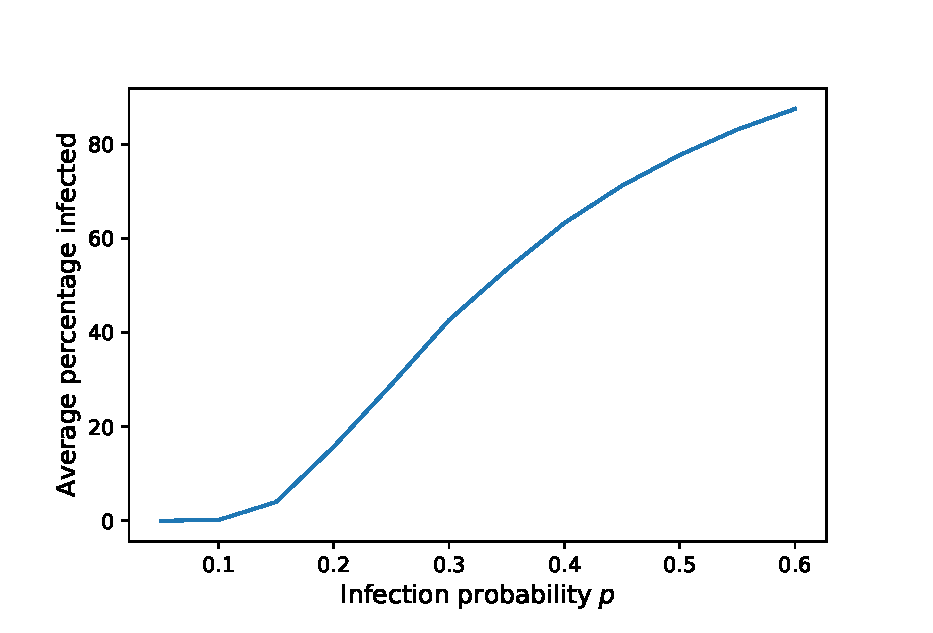
\includegraphics[scale = 0.55]{Figuresnew/PA_attackrates.eps}
    \caption{Preferential: p vs avg. percent infected.)}
    \label{fig:PA_ar}
\end{figure}

\begin{figure}[!h]
    \centering
    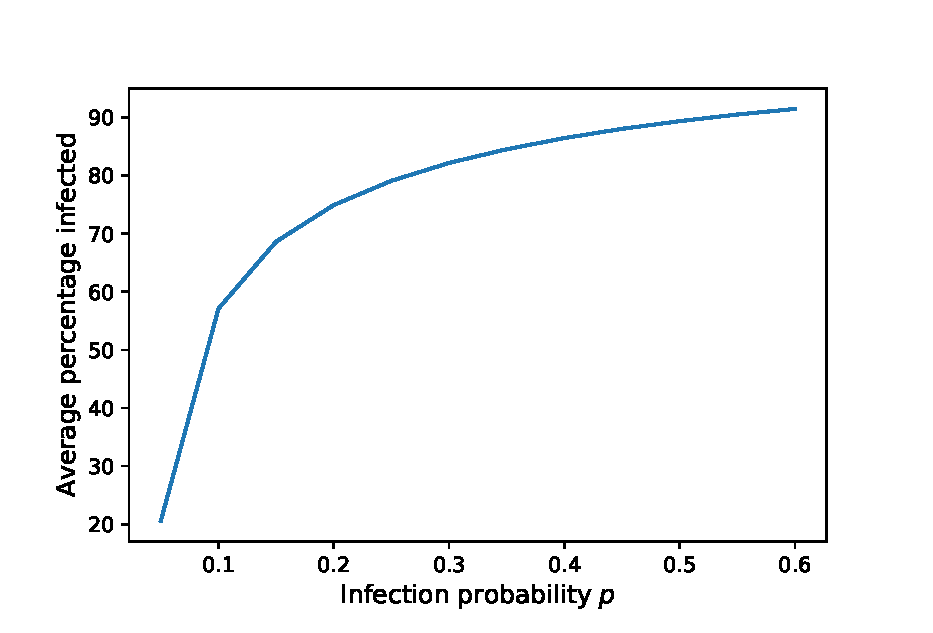
\includegraphics[scale = 0.55]{Figuresnew/montgo_attackrates.eps}
    \caption{Montgomery: p vs avg. percent infected.}
    \label{fig:montgo_ar}
\end{figure}



\begin{figure}[!h]
    \centering
    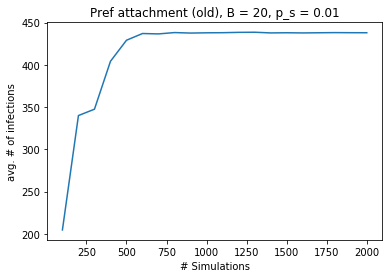
\includegraphics[scale = 0.6]{Figuresnew/simulations.png}
    \caption{Simulation vs average infected (Preferential Attachment)}
    \label{fig:pa_simvsavg}
\end{figure}
 
\begin{figure}[!h]
    \centering
    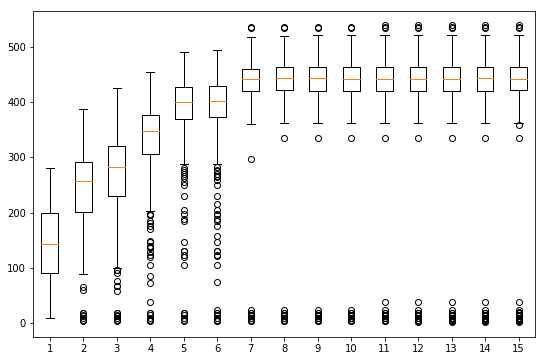
\includegraphics[scale = 0.45]{Figuresnew/boxplotpa.png}
    \caption{Box-plot: Simulation vs average infected (Preferential Attachment). X-axis: number of simulations (in 100s). Y-axis the number of infected.}
    \label{fig:pa_boxplot}
\end{figure}


\subsection{Approximation Guarantees}


\subsection{Characterizing Structure of Solution}

